%\documentclass[12pt]{article}
\documentclass[12pt,legalpaper]{article}
\usepackage{fullpage}
\usepackage{amsmath,amssymb}
\usepackage{mathptmx}
\usepackage{fancyhdr}
\usepackage{lastpage}
\usepackage{multicol}
\usepackage{graphicx}
\usepackage[aux]{rerunfilecheck}
\usepackage[rflt]{floatflt}

\setlength{\textheight}{11.5in}

\reversemarginpar

\newcommand{\myimp}{\Rightarrow}
\newcommand{\myiff}{\Leftrightarrow}
\newcommand{\mynot}{\neg}
\newcommand{\myor}{\vee}
\newcommand{\myand}{\wedge}
\newcommand{\ds}{\displaystyle}

\DeclareSymbolFont{AMSb}{U}{msb}{m}{n}
\DeclareMathSymbol{\N}{\mathbin}{AMSb}{"4E}
\DeclareMathSymbol{\Z}{\mathbin}{AMSb}{"5A}
\DeclareMathSymbol{\R}{\mathbin}{AMSb}{"52}
\DeclareMathSymbol{\Q}{\mathbin}{AMSb}{"51}
\DeclareMathSymbol{\I}{\mathbin}{AMSb}{"49}
\DeclareMathSymbol{\C}{\mathbin}{AMSb}{"43}

\pagestyle{fancy}
\lhead{MATH 110 S01 S02 200830                                             \\ 
  Final Examination \hspace{1.25in} Page\ \thepage\ of \pageref{LastPage}  \\ 
  Time: 3 hours                                                            \\
  \quad                                                                      }
%\chead{\quad                                                              \\ 
%       Page\ \thepage\ of \pageref{LastPage}                              \\ 
%	\quad                                                                }
\chead{}
\rhead{Name: \underline{\hspace{2in}}        \\ 
       Student \#: \underline{\hspace{2in}}  \\ 
       Section: \underline{\hspace{2in}}     \\
       \quad                                   }
\cfoot{}
\addtolength{\headheight}{\baselineskip}
\addtolength{\headheight}{\baselineskip}
\addtolength{\headheight}{\baselineskip}
\addtolength{\headheight}{\baselineskip}
\renewcommand{\headrulewidth}{0pt}
\fancypagestyle{plain}{%
  \lhead{}
  \chead{FIRST NATIONS UNIVERSITY OF CANADA  \\
    DEPARTMENT OF SCIENCE                    \\
    MATH 110--S01--S02 200830 \\
  }
  \rhead{}
  \cfoot{Page\ \thepage\ of \pageref{LastPage}}
}

\title{Final Examination}
\author{Edward Doolittle}

\begin{document}
\thispagestyle{plain}
%\maketitle

\begin{center}
  \LARGE{MATH 110--S01--S02 Final Examination 200830}
\end{center}

\begin{flushleft}
\quad\\
Time:  3 hours                  \hfill       Name: \underline{\hspace{2in}}  \\
Instructor:                     \hfill Student \#: \underline{\hspace{2in}}  \\
\quad Dr. Edward Doolittle  \hfill    Section: \underline{\hspace{2in}}  \\
\end{flushleft}


\noindent
You have 3 hours to do all of the following questions.
The test is worth a total of 100 marks.
Please\marginpar{\footnotesize{(marks)}} justify your conclusions and
show all your work.
A non-programmable calculator of the type mentioned in the course outline
is permitted; no other aids are permitted.
Use the backs of the pages for rough work.

\begin{enumerate}
\item Find\marginpar{\footnotesize{(10)}}
  $\ds \frac{dy}{dx}$ in each of the following cases.
  You do not have to simplify your answer.
  \begin{enumerate}
  \item $\ds y = x^5 - \frac{1}{x^{1/2}} + \tan(x^2)$
\vfill
  \item $\ds y = \frac{\cos(\sqrt{x})}{\sin x}$
\vfill
  \item $\ds x=\sin\left(xy\right)+y$
\vfill
  \item $\ds y=\int_2^{x} \frac{1}{t^2+1} \; dt$
\vfill
  \end{enumerate}
\newpage
\item Evaluate\marginpar{\footnotesize{(10)}}
  the following limits if they exist.
  \begin{enumerate}
  \item $\ds \lim_{x\to 0} \frac{x}{\sin \pi x}$
\vfill
  \item $\ds \lim_{x\to -\infty} \frac{4x^3-9x}{(3-x)(x^2+3)}$
\vfill
  \item $\ds \lim_{x\to 2^+} \frac{x^2-4}{x^2-4x+4}$
\vfill
  \item $\ds \lim_{x\to \infty} x-\sqrt{x^2+2x}$
\vfill
  \end{enumerate}
\newpage
\item A\marginpar{\footnotesize{(10)}} 
  piece of wire 10 m long is cut into two pieces.  One piece is bent
  into a square and the other is bent into a circle.  How should the wire
  be cut so that the total area enclosed is a maximum?  (Hint: the area $S$ of
  a square in terms of its perimeter $p$ is $A=(p/4)^2=p^2/16$; 
  the area $T$ of a circle in terms of its circumference $q$ 
  is $T=\pi(q/(2\pi))^2=q^2/(4\pi)$.)
\vfill
\newpage
\item Two\marginpar{\footnotesize{(10)}} cars start moving from the same
  point.  One travels south at 60 km/h and the other travels west at 25
  km/h.  At what rate is the distance between the cars increasing two
  hours later?
\vfill
\newpage
\item Consider\marginpar{\footnotesize{(12)}} the function $f$ given below
  along with its first and second derivatives.
  \begin{displaymath}
    f(x) = -\frac{(5x+7)(x+11)}{(1-x)^2}
    \qquad
    f'(x) = -\frac{72(x+3)}{(1-x)^3}
    \qquad
    f''(x) = -\frac{144(x+5)}{(1-x)^4}
  \end{displaymath}
  Fill in the blanks for parts (a) and (b).  Use the space below to show
  your work.  If more space is required use the back of the previous page
  and indicate that you have done so.
  \begin{enumerate}
  \item Identify all (if any)\\
    Intercepts \hrulefill\\
    Local extrema (max/min) \hrulefill\\
    Inflection points \hrulefill\\
    Asymptotes \hrulefill
  \item Determine the intervals on which $f$ is\\
    Increasing \hrulefill\\
    Decreasing \hrulefill\\
    Concave up \hrulefill\\
    Concave down \hrulefill\\
\vfill
\newpage
  \item Use the information in parts (a) and (b) on the previous page to
    sketch a graph of $f$.
  \end{enumerate}
\vfill
\newpage
\item Evaluate\marginpar{\footnotesize{(10)}}
  the following integrals.
  \begin{enumerate}
  \item $\ds \int\frac{(x+3)^2}{x^5} \; dx$
\vfill
  \item $\ds \int\frac{\sin x}{(4-\cos x)^2} \; dx$
\vfill
  \item $\ds \int_1^9 \sqrt{2x+7} \; dx$
\vfill
  \item $\ds \int_0^{1} \frac{x}{\sqrt{x^2+3}} \; dx$
\vfill
  \end{enumerate}
\newpage
\item Sketch\marginpar{\footnotesize{(10)}} 
  the region bounded by the curves $x+y=3$ and $y=x^2-2x-3$ and then
  find the area of the region.
\vfill
\newpage
\item Find\marginpar{\footnotesize{(8)}} 
  the tangent line to the curve
  \begin{displaymath}
    x^3+y^3+(x-y)^3=20
  \end{displaymath}
  at the point $(1,3)$ on the curve.
\vfill
\newpage
\item 
  \begin{enumerate}
  \item Calculate\marginpar{\footnotesize{(10)}} 
    $\ds\int_0^3 (x^2+x) \; dx$ from first principles, i.e., using
    the definition of a definite integral.
    (Note: you will receive no credit for 
    using the Fundamental Theorem of Calculus in this problem.)
    You may find some of the following formulas useful:
    \begin{displaymath}
      \sum_{i=1}^n i = \frac{n(n+1)}{2}
      \qquad
      \sum_{i=1}^n i^2 = \frac{n(n+1)(2n+1)}{6}
      \qquad
      \sum_{i=1}^n i^3 = \left(\frac{n(n+1)}{2}\right)^2
    \end{displaymath}
  \item Find a Riemann sum which estimates the integral in part (a).
    The sum should use $n=3$ equal intervals and should 
    use the right-hand endpoints of the intervals for sample points.
\vfill
  \end{enumerate}
\newpage
\item
  \begin{enumerate}
  \item Show\marginpar{\footnotesize{(10)}}
    that the equation $x^5+x+1 = 0$ has 
    \textbf{exactly} 
    one root in the interval $[-2,1]$.
\vfill
\vfill
\vfill
\vfill
  \item List the $x$ values at which the function graphed below 
    is not continuous.
\vfill
  \item List the $x$ values at which the function graphed below
    is continuous but not differentiable.
\vfill
    \begin{center}
      \includegraphics[width=6in]{cont.eps}
    \end{center}
  \end{enumerate}
\end{enumerate}
\end{document}

